\documentclass[12pt,bibliography=oldstyle,DIV=14,parskip=full-,titlepage]{scrartcl}
% esto me setea la variable pdf dependiendo del valor de \pdfoutput, que es >0
% sólo cuando estoy usando pdflatex para compilar el documento
%% \newif\ifpdf
%% \ifnum\pdfoutput<0
%% \pdffalse\fi
%% \ifnum\pdfoutput=0
%% \pdffalse\fi
%% \ifnum\pdfoutput>0
%% \pdftrue\fi


%
% ===
% === Trick para detectar si el documento está siendo compilado con pdflatex
% ===
%
% Esto me setea la variable pdf dependiendo del valor de \pdfoutput, que es >0
% sólo cuando estoy usando pdflatex para compilar el documento. Con esto puedo
% hacer  \ifpdf {...} \fi, que se ejecuta colo cuando compilo con pdflatex.
%% \newif\ifpdf
%% \ifnum\pdfoutput<0
%% \pdffalse\fi
%% \ifnum\pdfoutput=0
%% \pdffalse\fi
%% \ifnum\pdfoutput>0
%% \pdftrue\fi
%
% ===
% === I18n / L10n
% ===
%
% babel me da separación de sílabas para palabras en el idioma que le paso como
%       argumento opcional.
\usepackage[spanish,es-tabla,english]{babel}
%
% inputenc define la codificación de caracteres del código fuente, acá utf8.
\usepackage[utf8]{inputenc}
%
% ===
% === Gráficos
% ===
% 
% pst-pdf me permite usar PSTricks con pdflatex. Necesito cargarlo sólo si está
%         definida la variable pdf, por eso está entre \ifpdf ... \fi
%\ifpdf\usepackage{pst-pdf}\fi
%
% color me permite usar colores en el documento.
\usepackage{color}
%
% graphicx me da el comando \includegraphics para insertar imágenes (?)
\usepackage{graphicx}
%
% pstricks es un conjunto de macros basadas en PostScript para TeX, en
%          castellano: me da un entorno pstricks y comandos que uso dentro de
%          éste, que me sirven para dibujar figuras/diagramas/etc de manera
%          relativamente simple.
%\usepackage{pstricks}
%
% pst-circ me da macros para pstricks que me dibujan elementos de circuitos
%\usepackage{pst-circ}
%
% pst-plot me provee de funciones de ploteo para pstricks
%\usepackage{pst-plot}
%
% pst-2dplot me sirve para plotear en pstricks, entorno pstaxes
%\usepackage{pst-2dplot}
%
% ===
% === Verbatims
% ===
%
% verbatim es una reimplementación de los entornos verbatim[*]
%          provee el comando \verbatiminput{archivo} y el entorno comment, que
%          hace que LaTeX ignore directamente todo lo que está adentro
%\usepackage{verbatim}
%
% moreverb implementa el entorno verbatimtab indentando los tabs que encuentre,
%          y también el entorno listing, que pone números de línea al verbatim.
%          Para cambiar el ancho de la tabulacion, uso
%          \renewcommand\verbatimtabsize{<ancho del tab>\relax}
%          También define el entorno boxedverbatim.
%\usepackage{moreverb}
%
% listings me da el entorno lstlisting con resaltado de sintaxis.
%          Para setear el lenguaje del código, hago \lstset{language=<lang>}
%\usepackage{listings}
%
% url es un verbatim para escribir URL's que permite linebreaks dentro de ésta.
%     para usarlo, \url{<URL>}
\usepackage{url}
%
% ===
% === Más packages
% ===
%
%% \usepackage{mdwlist}		%Para listas mas compactas
%% \usepackage{textcomp}		%Para algunos símbolos
%% \usepackage{colortbl}		%Para celdas de colores en tablas
%% \usepackage{fancyhdr}		%Para encabezados/pie
\usepackage{bbold}		%Fuente bb para modo math: \mathbb{R} = reales
\usepackage{dsfont}		%Fuente ds para modo math: \mathds{R} = reales
\usepackage{multirow}		%Para "combinar" celdas en tablas
\usepackage{float}		%Para mejorar cuadros, figuras, etc
%% \usepackage{fancybox}		%Para recuardos de texto con bordes "fancy"
%% \usepackage{dingbat}		%Para dingbats
%\usepackage{marginal}		%Para  notas al margen que no puedo hacer andar
\usepackage{amsmath}		%Para enornos matemáticos mas flexibles
%\usepackage{varwidth}		%varwidth es un minipage que se ajusta al ancho mínimo


\usepackage[backend=biber,sorting=none,style=ieee,eprint=false,url=false]{biblatex} %% style=ieee
%% requiere texlive-bibtex-extra en debian


\usepackage{enumitem}
\setlist{noitemsep}
%% \setlist[description]{noitemsep}
%% \setlist[enumerate]{noitemsep}
%% \setlist[itemize]{noitemsep}

\usepackage{tikz}
\usepackage{pgfkeys}
\usepackage{pgfgantt}

% typearea: uso con koma-script para ajustar márgenes de página.
% vars globales a setear en la clase koma-script: DIV=12, BCOR=margen de ``binding'' para double side
\usepackage{typearea}

% para poder usar footnotes p.ej, adentro de un tabular
\usepackage{footnote}
\makesavenoteenv{tabular}

% para tabulars mas lindos/legibles
\usepackage{booktabs}

%\usepackage{glossaries}

\usepackage[spanish]{algorithm2e}

% para highlight (comando \hl{})
\usepackage{soulutf8}

% para teoremans etc
\usepackage{amsthm}

% para tunear citations
%\usepackage[square,comma,numbers,sort&compress]{natbib}


% config.tex: configuraciones del documento
%\selectlanguage{spanish}		%Elijo idioma español

%Permitir que los entornos equation, align, etc permitan saltos de página
%\allowdisplaybreaks[1]

%Tweaks
%% \setlength{\parindent}{0mm}		%Sangría de 1a. línea
%% \setlength{\hoffset}{2.6mm}		%
%% \setlength{\voffset}{-5.4mm}		%
%% \setlength{\topmargin}{0mm}		%
%% \setlength{\oddsidemargin}{5mm}	%
%% \setlength{\evensidemargin}{5mm}	%
%% \setlength{\marginparsep}{5mm}	%
%% \setlength{\headheight}{12.5mm}	%
%% \setlength{\headsep}{2.5mm}		%
%% \setlength{\footskip}{10mm}		%
%% \setlength{\textwidth}{14.1cm}		%
%% \setlength{\textheight}{232mm}	%
%% \setlength{\fboxrule}{.1pt}
%% \setlength{\parskip}{.5\baselineskip}

%Colores
\definecolor{negro}	{cmyk}{0,0,0,1}
\definecolor{marron}	{cmyk}{0,.5,1,.41}
\definecolor{rojo}	{cmyk}{0,1,1,0}
\definecolor{naranja}	{cmyk}{0,.35,1,0}
\definecolor{amarillo}	{cmyk}{0,0,1,0}
\definecolor{verde}	{cmyk}{1,0,1,0}
\definecolor{azul}	{cmyk}{1,1,0,0}
\definecolor{violeta}	{cmyk}{.45,1,0,0}
\definecolor{gris}	{cmyk}{0,0,0,.5}
\definecolor{blanco}	{cmyk}{0,0,0,0}
\definecolor{dorado}	{cmyk}{0,.16,1,0}
\definecolor{plateado}	{cmyk}{0,0,0,.25}

%% \title{\titulo}
%% \author{\autor}
%% \date{\fecha}

% si uso pdflatex, me setea las propiedades del pdf de salida
%% \ifpdf\pdfinfo{/Title    (\tituloPDF)
%%                /Author   (\autorPDF)
%%                /Subject  (\asuntoPDF)
%%                /Keywords (\clavesPDF)}\fi

% comandos.tex
% en este archivo defino todos los comandos/environment que quiera usar en mi documento.
%
% ===
% === Comandos
% ===
% 
% T: para escribir texto común cuando en modo math
%    uso: \T{texto que aparecerá en letra normal}
\newcommand{\T}{\textrm}
%
% aclaracion: dibuja un recuadrito aclaratorio, como <quote> en HTML.
%             uso: \aclaracion{Texto...}
\newcommand{\aclaracion}[1]{%
\smallpencil\-\begin{minipage}{0.9\textwidth}
%\vspace*{6pt}
{#1}\smallskip\end{minipage}}
%
% consigna: parecido a aclaración, pero con texto _slanted_
%           uso: \consigna{Consigna...}
\newcommand{\consigna}[1]{%
\leftpointright\ \parbox[t]{0.9\textwidth}{\textsl{#1}\vspace{8pt}}}
%
% pinterno: para representar el producto interno entre los dos argumentos
%           uso: \pinterno{X}{Y}
\newcommand{\pinterno}[2]{%
\left\langle #1 , #2 \right\rangle}
%
% === Estilos de texto
%
% resalt: resaltado con fondo verde
%         uso: \resalt{texto resaltado}
\newcommand{\resalt}{\colorbox{yellow}}
%
% sfbf: texto en negrita + slanted
%       uso:
\newcommand{\sfbf}[1]{\textsf{\bfseries #1}}
%
% small bold sans-serif
\newcommand{\sbs}[1]{\textsf{\small\bfseries #1}}
%
% eng: itálica (para palabras en inglés)
%      uso: \eng{some English text}
\newcommand{\eng}{\textit}
%
% mean: significado de una sigla - slanted
%       uso: (...) SNCF: \mean{Société Nationale des Chemins de Fer Francais} ...
\newcommand{\mean}{\textsl}
\newcommand{\desc}{\textsl}
%
% defin: pone en negrita el texto, útil para definiciones
%        uso: \defin{asshole}: vulgar slang for anus
\newcommand{\defin}{\textbf}
%
% R, N: cambia la tipografía en modo math, probar para ver cómo quedan
%       uso: \R{R} , \N{N}
\newcommand{\R}{\mathds}
\newcommand{\N}{\mathbf}
\newcommand{\C}{\mathcal}
\newcommand{\B}{\boldsymbol}
%
% dx: para escribir d2y/dx2, etc
\newcommand{\dx}[2]{\frac{d^{#2}\!#1}{d\!x^{#2}}}
%
% dp: para escribir derivadas parciales d2y/dx2, etc
\newcommand{\dpar}[3]{\frac{\partial^{#3}#1}{\partial{#2}^{#3}}}
%
% dvar: para escribir derivadas totales d2y/d(VAR)2, etc
\newcommand{\dvar}[3]{\frac{d^{#3}#1}{d{#2}^{#3}}}
%
% evalen: para escribir (loquesea)|_{evaluado_en}
\newcommand{\evalen}[2]{\left.{#2}\right|_{#1}}
%
% lil: para escribir texto pequeño. más cómodo que { \footnotesize texto pequeño... }
%      uso: \lil{texto pequeño... }
\newcommand{\lil}[1]{\footnotesize #1}  %Para texto pequeñooo
%
% mono: escribe el texto que le paso como parámetro con letra de ancho fijo
%       uso: \mono{texto monoespaciado}
\newcommand{\mono}[1]{{\texttt{#1}}}
%
% === Símbolos
%
\newcommand{\y}{\wedge}			%Y (Lógica)
\newcommand{\ve}{\vee}			%O (Lógica)
\newcommand{\ent}{\supset}		%Entonces (Lógica)
\newcommand{\dimp}{\leftrightarrow}	%Doble implicativo, equivalencia (Lógica)
\newcommand{\sii}{\leftrightarrow}	%Si y sólo si (Lógica)
\newcommand{\equi}{\equiv}		%Equivalencia (Lógica)
\newcommand{\portanto}{\vdash}		%Por lo tanto (Lógica)
\newcommand{\por}{\cdot}		%Producto punto
\newcommand{\RR}[1][1]{\mathds{R}}	%R de reales
\newcommand{\hfi}{\hat{\phi}}           %fi con gorrito arriba
\newcommand{\bfi}{\bar{\phi}}           %fi con raya arriba
\newcommand{\hpsi}{\hat{\psi}}          %Letra griega psi con gorrito arriba
\newcommand{\II}{\B{I}}                 %w negrita
\newcommand{\KK}{\B{K}}                 %w negrita
\newcommand{\QQ}{\B{Q}}                 %w negrita
\newcommand{\YY}{\B{Y}}                 %w negrita
\newcommand{\Bg}{\B{g}}                 %w negrita
\newcommand{\nn}{\B{n}}                 %w negrita
\newcommand{\uu}{\B{u}}                 %w negrita
\newcommand{\vv}{\B{v}}                 %w negrita
\newcommand{\ww}{\B{w}}                 %w negrita
\newcommand{\xx}{\B{x}}                 %x negrita
\newcommand{\yy}{\B{y}}                 %y negrita
\newcommand{\zz}{\B{z}}                 %z negrita
\newcommand{\BPhi}{\B{\Phi}}            %\Phi negrita
\newcommand{\Balpha}{\B{\alpha}}        %\alpha negrita
\newcommand{\Bbeta}{\B{\beta}}          %\beta negrita
\newcommand{\Btheta}{\B{\theta}}        %\theta negrita
\newcommand{\Bxi}{\B{\xi}}              %\xi negrita
%
%
% ===
% === Environments
% ===
% 
% enunciado: un environment que básicamente tiene el mismo efecto que el
%            comando consigna.
%            uso: \begin{enunciado} ... contenido ... \end{enunciado}
\newenvironment{enunciado}
{\leftpointright\ \begin{varwidth}[t]{0.9\textwidth}\textsl}
{\end{varwidth}\vspace{8pt}}
%
% pvi: para tipear la definición de un problema de valor inicial/funciones
%      definidas de a trozos/etc directamente en el texto (sin necesidad de
%      cambiar a un modo matemático.
%      uso: \begin{pvi} linea1 \\ linea 2 \\ ... \end{pvi}
\newenvironment{pvi}{\begin{equation}\begin{cases}}
{\end{cases}\end{equation}}
%
% pvi*: comp pvi, pero sin número de ecuación
\newenvironment{pvi*}{\begin{equation*}\begin{cases}}
{\end{cases}\end{equation*}}
%
% verbatimsmall: un verbatim con letra más chica. usualmente queda bastante
%                mejor que el verbatim pelado.
%                uso: \begin{verbatimsmall} ........ \end{verbatimsmall}
\newenvironment{verbatimsmall}{\small\begin{verbatim*}}
{\end{verbatim*}}
%
% nota: escribe una aclaracion dentro del texto
\newenvironment{nota}{$$\left[\;\begin{minipage}{0.95\textwidth}\slshape}
{\end{minipage}\;\right]$$}
%
%
% ===
% === Comandos ``históricos''
% ===
%
%% %\begin{pspicture}
%% \def\tierra(#1){%Para dibujar el símbolo de tierra en el entorno PSTricks
%% 	\rput(#1){
%% 		\psdot(0,0)
%% 		\psline(0,0)(0,-0.45)
%% 		\psline(-0.5,-0.45)(0.5,-0.45)
%% 		\psline(-0.35,-0.6)(0.35,-0.6)
%% 		\psline(-0.2,-0.75)(0.2,-0.75)
%% 	}%
%% }
%% %\end{pspicture}

\newcommand{\codigo}[2]{%Para generar un recuadro con código
	%\setlength{\hrulewidth}{0.1pt}
	\begin{flushleft}
	\underline{#1}
	\begin{tabular}{@{\quad}|l}
		\begin{minipage}{.85\textwidth}\smallskip{#2}
	\end{minipage}\end{tabular}\end{flushleft}%
}

\newcommand{\filecodigo}[1]{%Insertar código verbatim desde un archivo
\codigo{#1}{\verbatiminput{#1}}}%Requiere el paquete verbatim
\newcommand{\filecodigobis}[1]{{\verbatiminput{#1}}}%Requiere el paquete verbatim

%% \newcommand{\grafico}[3][1]{%Para generar un plot de un archivo con coords.
%% %\def\deequis=#1
%% \begin{minipage}{0.5\textwidth}\begin{center}
%% \begin{pspicture}(6,5)
%% 	\psgrid[subgriddiv=1,gridlabels=0pt,gridwidth=.1pt](1,3)(1,1)(6,5)
%% 	\psset{xunit=5cm,yunit=2cm}
%% 	\fileplot[linewidth=1pt,linecolor=blue,origin={0.2,1.5}]{#2}
%% 	\psset{xunit=1cm,yunit=1cm}
%% 	\psaxes[Dx=#1,dx=5,Oy=-1,Dy=1,dy=2]{-}(0.9,1)(6,5)
%% 	\rput(4,0.4){\textsl{#3}}
%% \end{pspicture}\end{center}\end{minipage}}

%% \newcommand{\eqncode}[2]{%
%% \begin{center}
%% \begin{tabular}{l@{\hspace{0.5cm}}r}
%% \begin{minipage}{.4\textwidth}
%% \begin{equation*}
%% #1
%% \end{equation*}
%% \end{minipage}
%% &
%% \fbox{\begin{minipage}{.4\textwidth}
%% %\setlength{\parskip}{4mm}
%% \filecodigobis{#2}
%% \end{minipage}}
%% \end{tabular}
%% \end{center}
%% }

%% \newcommand{\eqncodeb}[2]{%
%% \begin{center}\begin{tabular}{l@{\hspace{0.5cm}}r}
%% \begin{minipage}{.4\textwidth}#1\end{minipage} &
%% \fbox{\begin{minipage}{.4\textwidth}\filecodigobis{#2}\end{minipage}}
%% \end{tabular}\end{center}}

%% \newenvironment{matemcode}[1]{\newline
%% \begin{tabular}{l@{\hspace{0.5cm}}r}
%% \begin{minipage}{.4\textwidth}
%% \parbox[t]{.4\textwidth}{\begin{equation*}#1\end{equation*}}\end{minipage}
%% &\begin{Sbox}\begin{minipage}{.4\textwidth}}
%% {\end{minipage}\end{Sbox}\fbox{\TheSbox}\end{tabular}\newline}

%% \newenvironment{encuadrar}[1]{\begin{Sbox}\begin{varwidth}{#1\textwidth}}
%% {\end{varwidth}\end{Sbox}\fbox{\TheSbox}}

%% \newenvironment{parboxenv}{\begin{Sbox}}
%% {\end{Sbox}\parbox[t]{.9\textwidth}{\TheSbox}}

% multicolumn y multirow
\newcommand{\mcol}[3]{\multicolumn{#1}{#2}{#3}}
\newcommand{\mrow}[3]{\multirow{#1}{#2}{#3}}

%% Serif .......................................................................
%%
%% New Century Schoolbook
%% \usepackage[T1]{fontenc}
%% \usepackage{fouriernc}
%%
%%
%% TeX Gyre Schola (New Century extendida)
%% \usepackage[T1]{fontenc}
%% \usepackage{tgschola}
%%
%%
%% Utopia
%% \usepackage[T1]{fontenc}
%% \usepackage{fourier}
%%
%%
%% Utopia (con MathDesign)
%% \usepackage[T1]{fontenc}
%% \usepackage[adobe-utopia]{mathdesign}
%%
%%
%% Computer Concrete
%% \usepackage[T1]{fontenc}
%% \usepackage{concmath}
%%
%%
%% Charter BT
 \usepackage[T1]{fontenc}
 \usepackage[bitstream-charter]{mathdesign}
%%
%%
%% Nimbus Roman (clon de Times)
%% \usepackage[T1]{fontenc}
%% \usepackage{nimbus}
%%
%%
%% TeX Gyre Termes (version mejorada de Nimbus Roman)
%% \usepackage[T1]{fontenc}
%% \usepackage{tgtermes}
%%
%%
%% GFS Bodoni
%% \usepackage[T1]{fontenc}
%% \usepackage[default]{gfsbodoni}
%%
%%
%% Baskervald ADF
%% \usepackage[T1]{fontenc}
%% \usepackage{baskervald}
%%
%%
%% Efont Serif -- descargar de http://openlab.jp/efont/serif/
%% \usepackage[T1]{fontenc}
%% \usepackage{efont,mathesf}
%% \renewcommand*\oldstylenums[1]{{\fontfamily{esfod}\selectfont#1}}
%%
%%
%%
%%
%%
%% Sans-Serif ..................................................................
%%
%%
%% Optima (clon de, URW Classico)
%% \usepackage[T1]{fontenc}
%% \renewcommand*\sfdefault{uop}
%%
%%
%% Avantgarde (clon de, URW Gothic)
%% \usepackage[T1]{fontenc}
%% \usepackage{avant}
%%
%%
%% TeX Gyre Adventor (version mejorada de Avantgarde)
%% \usepackage[T1]{fontenc}
%% \usepackage{tgadventor}
%%
%%
%% Nimbus Sans (clon de Helvetica)
%% \usepackage[T1]{fontenc}
%% \usepackage{nimbus}
%%
%%
%% Helvetica (clon de, Nimbus Sans)
%% \usepackage[T1]{fontenc}
%% \usepackage[scaled]{helvet}
%%
%%
%% TeX Gyre Heros (version mejorada de Nimbus Sans)
%% \usepackage[T1]{fontenc}
%% \usepackage{tgheros}
%%
%%
%% Boilinum
%% \usepackage[T1]{fontenc}
%% \usepackage{libertine}
%%
%%
%% Computer Modern Bright
%% \usepackage[T1]{fontenc}
%% \usepackage{cmbright}
%%
%%
%% Latin Modern Sans
%% \usepackage[T1]{fontenc}
%% \usepackage{lmodern}
%%
%%
%% Epigrafica
%% \usepackage[OT1]{fontenc}
%% \usepackage{epigrafica}
%%
%%
%%
%% Si quiero el documento en sans en vez de Roman:
%% \renewcommand*\familydefault{\sfdefault}
%% ...............................................
%% 
%%
%%
%% Monospaced ..................................................................
%%
%%
%% Pandora Typewriter
%% \usepackage[T1]{fontenc}
%% \usepackage{pandora}
%%
%%
%% Letter Gothic
%% \usepackage[T1]{fontenc}
%% \usepackage{ulgothic}
%%
%%
%% Inconsolata
%% \usepackage[T1]{fontenc}
%% \usepackage{inconsolata}
%%

%
%
%
\selectlanguage{spanish}
\hyphenation{micro-RNA}
\hyphenation{micro-RNAs}
\hyphenation{mi-RNA}
\hyphenation{mi-RNAs}
%
%
%
\setkomafont{subject}{\LARGE\usekomafont{disposition}}
\setkomafont{title}{\normalfont\slshape}
%
\raggedbottom
%
\begin{document}
\selectlanguage{spanish}
%
\titlehead{\center\large Universidad Nacional del Litoral\\
  Facultad de Ingeniería y Ciencias Hídricas}
%
\subject{Propuesta de Proyecto Final de Carrera\\Ingeniería en
  Informática}
%
\title{\LARGE ``Desarrollo de un clasificador de secuencias de pre-microRNA
  mediante técnicas de Inteligencia Computacional''}
%
%\subtitle{hola que tal}
%
\author{{Alumno: Mauro Javier Torrez}\and{Director: Dr. Diego. H. Milone}}
%
%\publishers{Director: Dr. Diego H. Milone}
\date{\-\\[2em]\today}
\renewcommand*{\titlepagestyle}{empty}
\maketitle
\setcounter{page}{1}
%
%
\section{Título del Proyecto}
Desarrollo de un clasificador de
secuencias de pre-microRNA mediante
técnicas de Inteligencia Computacional
%
%
\section{Palabras clave}
miRNA, pre-miRNA, máquina de vectores
de soporte, perceptrón multicapa, clasificación
%
%
\section{Justificación}
%
%\subsection*{Descripción de los miRNAs y pre-miRNAs}
%
Hace aproximadamente una década se propuso que un tipo de pequeñas
moléculas previamente ignoradas, aunque presentes en grandes
cantidades en la célula, jugarían un papel decisivo en la reproducción
celular, promoviendo su diferenciación en distintos tipos de tejidos
y/o su permanencia en un estado particular de diferenciación
\cite{lee-mammal}.  Estas pequeñas moléculas de ácido ribonucleico
(\eng{RNA}, del inglés \emph{ribonucleic acid}), de unos 22
nucleótidos [nt] de longitud, se denominaron en inglés \eng{microRNA} o
\eng{miRNA}.  En trabajos posteriores se ha demostrado que los miRNA
ejercen una función reguladora de la expresión génica celular
\cite{bartel116} y están involucrados en varios procesos genéticos
dentro de la célula, como la transcripción de mRNA (\emph{RNA
  mensajeros}) y la síntesis de proteínas \cite{lili}.  Este efecto
regulador puede tener gran implicancia en el desarrollo y evolución de
la enfermedad celular. Se ha demostrado que los miRNA juegan un rol
importante en la carcinogénesis \cite{aurora}\cite{lili}, regulando la
proliferación y muerte celular, entre otras funciones como el
metabolismo de las grasas en moscas, los procesos de infección viral,
y el control del desarrollo de flores y hojas en plantas
\cite{bartel116}\cite{lecellier}.

Los miRNA se presentan naturalmente dentro de una molécula denominada
pre-miRNA o \emph{miRNA precursor}, de unos 70 nucleótidos de
longitud, la cual contiene uno o más miRNA \emph{maduros} en su
secuencia. En la Figura \ref{horquilla} se representa en forma
esquemática la secuencia de una cadena de pre-miRNA y su
correspondiente \emph{estructura secundaria}. Esta estructura
secundaria viene dada por la forma en que la cadena de pre-miRNA se
\emph{pliega} sobre sí misma logrando una mayor estabilidad
molecular. Tal como se aprecia en la figura, se encuentra que en el
reino animal la estructura secundaria de un pre-miRNA conforma una
especie de \emph{horquilla} \cite{bartel116}\cite{sewer}.
\begin{figure}[H]
\smallskip\small\slshape\center
  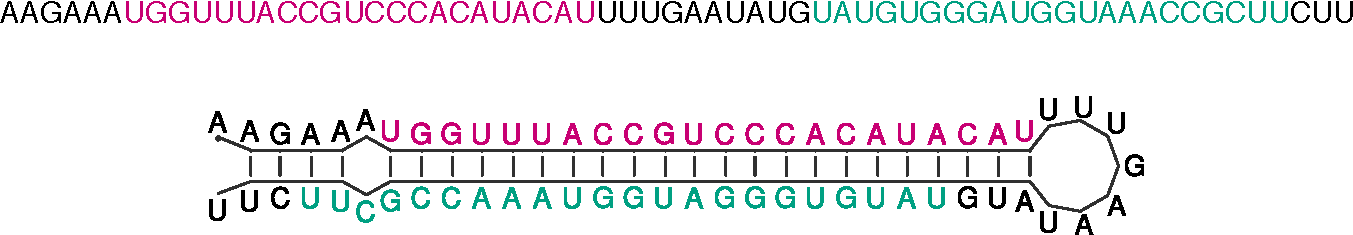
\includegraphics[width=.85\textwidth]{res/hsa-mir-299_ss.pdf}
  \caption{\small\slshape Secuencia
    (arriba) y estructura secundaria tipo horquilla (abajo) del
    pre-miRNA \textbf{hsa-mir-299}.  }
  \label{horquilla}
\end{figure}

El debate acerca del número e identidad de los miRNA presentes en
diferentes genomas es una cuestión abierta: a modo de ejemplo, para el
caso del genoma humano se había estimado inicialmente que se
encontrarían unos pocos cientos de genes miRNA; posteriormente este
número ha sido revisado a unos 1000 \cite{sewer}\cite{chang}.
Actualmente, se encuentra que el número de miRNAs descubiertos en
humanos duplica esta cifra \cite{gomes}.  Teniendo en cuenta que estas
predicciones consideran sólo aquellos miRNA que se encuentran
conservados entre especies relativamente distantes (como primates y
roedores) y no aquellos de evolución más reciente \cite{sewer}, el
número de miRNAs en humanos podría ser mucho mayor que las
estimaciones. La base de datos miRBase \cite{mirbase2}\cite{mirbase3}
recopila el conjunto de (pre-)miRNA conocidos hasta la
fecha. En la última versión disponible (r.19, agosto de 2012) se listan
21264 pre-miRNA experimentalmente validados, conteniendo un total de
25141 miRNA maduros, para 193 especies diferentes.
%

En principio, la identificación de nuevos miRNA se realiza en forma
experimental en el laboratorio. Ésta es la primera elección, pero sólo
aquellos miRNA abundantes pueden ser detectados de forma fiable
mediante esta técnica. Sin embargo, no todos los miRNAs están bien
expresados en múltiples tipos de tejidos: aquellos miRNA que tienen un
bajo nivel de expresión, que se expresan en tejidos específicos y/o
que se presentan sólo en determinados estadíos de desarrollo celular
pueden ser fácilmente ignorados mediante la técnica
experimental\cite{ding}\cite{xu}.  En pos de superar estas
dificultades propias del método experimental es que surgen técnicas
computacionales para encontrar aquellos miRNA que son específicos a
determinados tipos de tejidos o estadíos de desarrollo celular, y
aquellos escasamente expresados \cite{sheng}\cite{xu}.

Los métodos computacionales para el reconocimiento de genes miRNA se
han desarrollado en dos direcciones principales: los métodos
comparativos, basados en la conservación ya sea de la secuencia y/o la
estructura secundaria entre distintas especies, y los no-comparativos,
basados en el aprendizaje de máquina o Inteligencia
Computacional. Estos dos enfoques se complementan mutuamente al
encarar distintas estrategias para la predicción de nuevos miRNAs
\cite{batuwita}\cite{sheng}.

En un enfoque comparativo, se analizan genomas de diferentes especies
buscando correspondencias que cumplan con las características de un
pre-miRNA. Tal como en el caso del método experimental, mediante esta
técnica sólo es posible detectar aquellos pre-miRNAs conservados entre
especies y con un elevado nivel de expresión. En cambio, en un enfoque
no-comparativo se utiliza alguna técnica de aprendizaje de máquina,
para generar un modelo computacional que describe internamente las
características del pre-miRNA a partir de un conjunto de datos que se
utilizan en la etapa del entrenamiento. Con este modelo computacional
se genera un \emph{clasificador}.

El objetivo último de un clasificador no-comparativo es obtener una
tasa mínima de errores de clasificación para conjuntos de datos
nuevos, que no hayan sido utilizados en la etapa de entrenamiento.  En
Inteligencia Computacional se pueden utilizar diversas técnicas para
la implementación de un clasificador no-comparativo, entre ellas las
más utilizadas han sido el \emph{Perceptrón Multicapa}
\cite{mlp1}\cite{mlp2} y la \emph{Máquina de Vectores de Soporte}
\cite{svm}.  El Preceptrón Multicapa (\emph{MLP}, del inglés
\eng{Multilayer Perceptron}) es un tipo de red neuronal artificial con
propagación hacia adelante, donde las neuronas se disponen en capas.
La salida de cada neurona se determina al aplicar una \emph{función de
  activación}, de tipo sigmoidea, a la suma ponderada de las salidas
en la capa anterior. Durante el entrenamiento del MLP se ajustan los
pesos de cada neurona mediante un algoritmo de aprendizaje basado en
la \emph{retropropagación} del error de clasificación, hasta obtener
una tasa de clasificación satisfactoria \cite{jain}.  La Máquina de
Vectores de Soporte (\emph{SVM}, de su nombre en inglés \eng{Support
  Vector Machine}) es un algoritmo de clasificación que se basa en
transformar, mediante una función de mapeo llamada \emph{núcleo}, el
espacio $N$-dimensional de los datos de entrada en otro espacio de
dimensión $M: M\gg N$, donde se espera que los datos sean linealmente
separables mediante un hiperplano. El entrenamiento consiste en
encontrar el hiperplano óptimo de separación para el conjunto de datos
presentado \cite{bottou}.

En el Centro de Investigación en Señales, Sistemas e Inteligencia
Computacional \emph{sinc(i)} de la Facultad de Ingeniería y Ciencias
Hídricas surge la necesidad de contar con un clasificador de
pre-miRNA. Al revisar los desarrollos publicados en el tema, se
encuentra que en muchos casos las tasas de clasificación no son
satisfactorias, en otros casos, se obtienen buenas tasas de
clasificación sólo en casos particulares.  También se encuentra que en
muchos de los trabajos disponibles no se publica el código fuente, y
en los casos que se encuentran disponibles, están codificados en
lenguajes diferentes lenguajes, o bien funcionan con diferentes
formatos de entrada/salida.  Teniendo en cuenta estos inconvenientes
es que se propone en este trabajo desarrollar un método informático
para la identificación de pre-miRNAs mediante un clasificador de tipo
no-comparativo, que haga uso de técnicas de Inteligencia Computacional
para el reconocimiento de patrones.  Se integrarán técnicas que se
encuentran en la bibliografía con el propósito de obtener un
clasificador con una buena tasa de clasificación, con una interfaz
sencilla de cara al usuario no experto.

Para cada entrada presentada, el clasificador deberá ser capaz de
discriminar entre dos \emph{clases}: positiva para aquellas que
corresponden a un pre-miRNA y negativa para aquellas entradas que no
lo son. 
Una secuencia de pre-miRNA se representa mediante una cadena de
caracteres \mono{A, G, C, U,} donde cada carácter representa el tipo
de \emph{base} constitutiva de cada nucleótido\footnote{Las bases
  constitutivas del ARN son: \emph{adenina}, \emph{guanina},
  \emph{citosina} y \emph{uracilo}, de ahí la representación \mono{A, G,
    C, U}.}.
A partir de esta secuencia, mediante un proceso de extracción de
características se generará un vector numérico que será la entrada al
clasificador.  El sistema clasificará los datos de entrada
identificando aquellas secuencias candidatas a ser pre-miRNAs.  Se
desarrollarán clasificadores basados en MLP y SVM, comparando su
rendimiento, y se tomará en consideración la pertinencia de incluir
éstas y otras técnicas en el clasificador final.

Se seleccionarán conjuntos de datos tanto positivos como negativos
para el entrenamiento del clasificador. Como conjunto de datos
positivos, se deberán utilizar pre-miRNAs validados experimentalmente.
Para el caso negativo, se deberán utilizar datos artificialmente
seleccionados que no contengan pre-miRNAs, aunque sí presenten
características similares a éstos.

El impacto social del desarrollo de este proyecto se verá en un
aumento en la productividad de los investigadores del área al
posibilitarle una mayor facilidad de acceso que los sistemas actualmente
disponibles. También se pretende que sirva como puntapié inicial en
desarrollos futuros de sistemas similares con mayor complejidad y
rendimiento. En una visión englobadora, se agilizará la investigación
en el área con las implicancias que esto trae a la sociedad en
general, como el desarrollo de nuevos métodos de prevención y
tratamiento de enfermedades de diversa índole en las personas,
animales y plantas; y una mayor y mejor comprensión de los procesos
involucrados en su aparición y desarrollo.

El alumno considera que en lo personal, el desarrollo de este proyecto
le permitirá profundizar su conocimiento en diferentes áreas de la
Inteligencia Computacional, así como su aplicación al campo de la
bioinformática. Expresa que el desarrollo de este proyecto le
permitirá desarrollar habilidades y conocimientos que le serán de gran
valor en el desempeño como profesional, y en caso de seguir una
carrera de investigación servirá de introducción informal a la
metodología de trabajo en este campo.
%
%
\section{Objetivo general del proyecto}
Desarrollar un método computacional inteligente con interfaz de
usuario para la identificación de secuencias de RNA candidatas a ser
pre-miRNAs.
\section{Objetivos específicos}
\begin{itemize}
\item Generar una base de datos de pre-miRNAs conocidos en plantas y
  animales, armonizando los conjuntos de características entre las
  distintas bases de datos disponibles.
\item Codificar diferentes métodos de inteligencia computacional para
  trabajar sobre los datos. Se trabajarán al menos dos, SVM y MLP con
  la posibilidad de incorporar otros conforme se avance en este
  objetivo.
\item Comparar el rendimiento de los distintos métodos buscando
  obtener el mejor desempeño en la tasa de clasificación.
\item Especificar y codificar una interfaz de línea de comandos y una
  interfaz web para la utilización del método por parte del usuario no
  experto.
\end{itemize}
%
%
\section{Alcances}
\begin{itemize}
\item El trabajo se centrará en la utilización de algoritmos de
  clasificación de tipo Máquina de Vector de Soporte (SVM) y
  Perceptrón Multicapa (MLP), comparando el rendimiento de cada uno.
\item El sistema contará además con una interfaz de usuario
  documentada tal que éste sea accesible a los usuarios no expertos.
\item Se trabajará durante el desarrollo exclusivamente con datos de
  distintos organismos que se encuentren disponibles en línea, ya
  clasificados y validados experimentalmente.
\item Se utilizarán únicamente técnicas de extracción de
  características disponibles en la bibliografía.
\item En el sistema se trabajará únicamente con la identificación de
  pre-miRNAs, quedando fuera del alcance de este proyecto la
  identificación de el/los miRNAs ``maduros'' contenidos en éstos.
\end{itemize}
%
%
\section{Metodología a emplear}
El desarrollo del proyecto se llevará a cabo siguiendo un modelo de
ciclo de vida en cascada según las etapas que se enumeran a
continuación.  Cabe notar que, si bien estas etapas proveen una
separación lógica de tareas a tomar como referencia, no implican
necesariamente un orden cronológico de tareas a realizar. Así también,
debido a la naturaleza del proyecto se contempla la posibilidad de una
retroalimentación entre etapas, pudiendo retroceder a una fase
anterior si así es requerido.
%
\subsection{Estudio del estado del arte y herramientas informáticas
  disponibles}
Se procederá a recopilar y estudiar la bibliografía referente al tema
y se determinarán los métodos de clasificación y de extracción de
características disponibles. También se estudiarán las diferentes
herramientas de desarrollo y lenguajes disponibles tomando en
consideración factores como requerimientos de hardware/software,
disponibilidad, rendimiento, portabilidad y facilidad de uso.
%
\subsection{Especificación de requerimientos y pruebas iniciales}
Se realizará una búsqueda de datos disponibles en Internet a partir de
la bibliografía consultada.  Se codificarán varios métodos de
clasificación y se probarán sobre una de las bases de datos
encontradas para obtener una mejor comprensión de los requerimientos
del sistema.
%
Se evaluarán las herramientas informáticas disponibles para la
implementación y se especificarán aquellas a utilizar según los
resultados obtenidos en las pruebas iniciales.
%
\subsection{Preparación de los datos y codificación de partes del sistema}
Se recopilará el conjunto de datos encontrados en la etapa anterior y
se realizará un análisis exhaustivo de éstos.  Se codificarán
herramientas auxiliares para la extracción de características si fuera
necesario para lograr completitud y uniformidad de los diferentes
conjuntos de datos.  Se preparará una base de datos propia mediante la
selección, limpieza y adecuaciones de formato en cuanto sea necesario
con el objetivo de garantizar la calidad de la misma. Esta base de
datos contendrá secuencias de pre-miRNAs conocidos y validados
experimentalmente así como de secuencias que no sean pre-miRNAs
(ejemplos negativos) para utilizar en el entrenamiento y prueba del
clasificador.

El algoritmo de clasificación se desarrollará siguiendo
aproximadamente un modelo de prototipos. En forma iterativa se
realizarán pruebas sobre los clasificadores disponibles variando sus
parámetros y distintas características de entrada. Cada caso se
evaluará mediante validación cruzada obteniendo medidas de
rendimiento. A partir de estas medidas de rendimiento se especificarán
los algoritmos a utilizar en la parte de clasificación, con sus
parámetros correspondientes. Con esta especificación se procederá a la
codificación del algoritmo de clasificación definitivo.
%
\subsection{Integración del sistema e interfaz de usuario}
Se definirá el formato de los datos de entrada del sistema final y se
codificará un sistema integrado que incorpore extracción de
características y clasificación. Se seleccionarán los parámetros de
clasificación disponibles (configurables) al usuario final así como
valores por defecto que aseguren un buen rendimiento.
%
Se especificará y codificará una interfaz de usuario de línea de
comandos y una interfaz web, previa evaluación y selección de las
tecnologías a utilizar para la implementación.  Se generará la
documentación correspondiente para la utilización del sistema por
parte del usuario final.
%
\subsection{Pruebas finales y puesta en servicio}
En esta etapa se procederá a evaluar el sistema, verificando el buen
funcionamiento y el cumplimiento de los requerimientos. Se realizarán
pruebas de clasificación para obtener medidas de rendimiento
globales. Mediante pruebas se intentará encontrar y eliminar
aquellos fallos que pudieren haber sido pasados por alto durante el
desarrollo.
%
Finalmente, se procederá a la configuración de un servidor web de
ejemplo y se realizará la puesta en servicio del sistema sobre el
mismo, evaluando y especificando las tecnologías a utilizar para tal
fin.
%
%
\section{Plan de tareas propuesto}
Para el desarrollo del proyecto, el alumno dedicará 20 horas semanales
de trabajo para un total de 740 horas.  Se realizarán 2
reuniones mensuales de una hora con el director de proyecto para
seguimiento de avance y asesoramiento.
%
A continuación se presenta la lista de tareas y sub-tareas a
desarrollar en el transcurso del proyecto.
\begin{enumerate}
\item Búsqueda bibliográfica (56h)
  \begin{enumerate}
  \item Información específica del problema en cuestión: descripción
    de los microRNAs, mecanismo y función, implicancias en el campo de
    la biología (32h).
  \item Perspectiva informática del tema: estructura de los datos de
    entrada, extracción de características, métodos de clasificación
    (24h).
  \end{enumerate}
\item Implementación inicial de métodos de clasificación (44h)
  \begin{enumerate}
  \item Búsqueda y verificación de una base de datos de prueba ya
    clasificada y con las características extraídas (12h).
  \item Codificación inicial de clasificadores para obtener una
    primera impresión de las herramientas y lenguajes disponibles,
    requerimientos de software y hardware, y rendimiento (32h).
  \end{enumerate}
\item Preparación de la base de datos (76h)
  \begin{enumerate}
  \item Búsqueda y verificación de diferentes bases de datos (16h).
  \item Armado de una base de datos propia unificando el formato y
    características disponibles (32h).
  \item Codificación de herramientas para validación de la base de
    datos generada y pruebas (28h).
  \end{enumerate}
\item Redacción del informe entregable 1 (16h)
\item Diseño del clasificador definitivo (124h)
  \begin{enumerate}
  \item Pruebas de los clasificadores preliminares (80h).\\
    Tarea iterativa:
    \begin{itemize}
    \item Selección del método de clasificación.
    \item Ajuste de parámetros del método.
    \item Validación cruzada.
    \end{itemize}
  \item Codificación definitiva del clasificador (44h).
  \end{enumerate}
\item Pruebas e integración del sistema (104h)
  \begin{enumerate}
  \item Validación del método de clasificación (24h).
  \item Integración del sistema: extracción de características y
    clasificación (32h).
  \item Especificación y codificación de la interfaz de usuario de
    línea de comandos (24h).
  \item Pruebas de funcionamiento y validación de requerimientos (24h).
  \end{enumerate}
\item Redacción del informe entregable 2 (16h)
\item Interfaz de usuario web, documentación y puesta en servicio (132h)
  \begin{enumerate}
  \item Especificación de los lenguajes/tecnologías a utilizar en la
    interfaz web (16h).
  \item Codificación de la interfaz web (48h).
  \item Documentación de las interfaces de usuario de línea de
    comandos y web (24h).
  \item Configuración y puesta en servicio de un servidor de prueba
    (44h).
  \end{enumerate}
\item Redacción del informe entregable 3 (16h)
\item Redacción del informe final (156h)
\end{enumerate}
%
%
\section{Puntos de control y entregables}
\subsection{Punto de control 1}
Resultados de la revisión bibliográfica, pruebas preliminares y armado
de la base de datos definitiva.  Abarca las etapas 1 y 2 y la primera
parte de la etapa 3.
\begin{description}
  \item[Fecha:] 7 de agosto de 2013
  \item[Entregable:]
  \item
    \begin{minipage}{\textwidth}
      \medskip
      \begin{itemize}
      \item Bibliografía consultada
      \item Bases de datos recopiladas
      \item Métodos de clasificación codificados y pruebas preliminares
      \item Auxiliares de extracción de características codificados
      \item Armado de la base de datos definitiva
      \end{itemize}
    \end{minipage}
\end{description}

\subsection{Punto de control 2}
Resultados de la implementación del clasificador definitivo e
integración del sistema. Abarca la segunda parte de la etapa 3 y la
etapa 4 excepto la interfaz web y la documentación para el usuario
final.
\begin{description}
  \item[Fecha:] 31 de octubre de 2013
  \item[Entregable:]
  \item
    \begin{minipage}{\textwidth}
      \medskip
      \begin{itemize}
      \item Resultados de las pruebas de los distintos clasificadores
      \item Especificación del algoritmo de clasificación definitivo:
        métodos seleccionados, parámetros, conjunto de características
        considerado
      \item Algoritmo de clasificación codificado
      \item Resultados de la validación del algoritmo de clasificación
      \item Codificación del sistema integrado
      \item Interfaz de usuario de línea de comandos codificada
      \item Resultados de la validación de requerimientos
      \end{itemize}
    \end{minipage}
\end{description}
\subsection{Punto de control 3}
Interfaz de usuario web, puesta en servicio y documentación para el
usuario final. Abarca parte de la etapa 4 y la etapa 5.
\begin{description}
  \item[Fecha:] 7 de enero de 2014
  \item[Entregable:]
  \item
    \begin{minipage}{\textwidth}
      \medskip
      \begin{itemize}
      \item Documentación de la interfaz de línea de comandos
      \item Tecnologías web seleccionadas para la interfaz de usuario
      \item Interfaz de usuario web codificada
      \item Documentación de la interfaz de usuario web
      \item Servidor de prueba puesto en servicio
      \end{itemize}
    \end{minipage}
\end{description}
%
%
\section{Cronograma tentativo}
En el siguiente cronograma se distribuye la carga de trabajo de 740
horas en 37 semanas. Se toma como fecha de inicio del proyecto el día
3 de junio de 2013 y como fecha de finalización estimada el día 28 de
febrero de 2014. Se consideran como no laborables las dos semanas
comprendidas entre el día 23 de diciembre y 3 de enero.
\begin{center}
\definecolor{barblue}{RGB}{153,204,254}
\definecolor{groupblue}{RGB}{51,102,254}
\definecolor{linkred}{RGB}{165,0,33}
\sffamily
\begin{ganttchart}[
y unit chart=5mm,
x unit=0.75mm,
y unit title=6mm,
hgrid style/.append style={draw=black!5, line width=.75pt},
vgrid={*4{draw=black!15, line width=.75pt},%
  *1{draw=black!40, line width=.75pt}},
canvas/.append style={fill=none, draw=black!40, line width=.75pt},
include title in canvas=true,
title height=1,
title/.append style={draw=black!40, line width=.75pt,fill=none},
title label font=\bfseries\footnotesize,
bar label font=\mdseries\small\color{black!70},
bar incomplete/.append style={fill=black!63},
bar height=.6,
%bar label node/.append style={left=2cm},
bar/.append style={draw=none, fill=barblue},
progress label text=,
group incomplete/.append style={fill=groupblue},
group left shift=0,
group right shift=0,
group top shift=.3,
group height=.6,
group/.append style={shape=ganttbar},
milestone/.append style={shape=ganttmilestone,fill=linkred,draw=none},
milestone label font=\slshape\bfseries\small\color{black!80},
milestone height=.55,
milestone top shift=.35,
milestone left shift=-1,
milestone right shift=2,
milestone label node/.append style={below=8pt,left=0pt},
]{1}{185}
\gantttitle{Jun}{20}\gantttitle{Jul}{23}\gantttitle{Ago}{22}
\gantttitle{Sep}{21}\gantttitle{Oct}{23}\gantttitle{Nov}{21}
\gantttitle{Dic}{15}\gantttitle{Ene}{20}\gantttitle{Feb}{20}\\
\gantttitle[title label node/.append style={below left=-1.15ex and -1.1ex},
  title label font=\bfseries\scriptsize]{Semana:\quad\,1}{5}%
\gantttitlelist[title label font=\bfseries\scriptsize]{2,...,37}{5} \\
% 20 horas semanales: 1 dia = 4h
\ganttgroup{Tarea 1}{1}{14} \\%14 dias
\ganttbar{1.a}{1}{8} \\ %32h
\ganttbar{1.b}{9}{14} \\ %24h
%
\ganttgroup{Tarea 2}{15}{25} \\%11 dias
\ganttbar{2.a}{15}{17} \\ %12h
\ganttbar{2.b}{18}{25} \\ %32h
%
\ganttgroup{Tarea 3}{26}{44} \\%19 dias
\ganttbar{3.a}{26}{29} \\%16h
\ganttbar{3.b}{30}{37} \\%32h
\ganttbar{3.c}{38}{44} \\%28h
% entregable 1
\ganttgroup{Tarea 4}{45}{48} \\%4 dias
\ganttmilestone{Control 1}{48}\\
%
\ganttgroup{Tarea 5}{49}{79} \\%31 dias
\ganttbar{5.a}{49}{68} \\%80h
\ganttbar{5.b}{69}{79} \\%44h
%
\ganttgroup{Tarea 6}{80}{105} \\%26 dias
\ganttbar{6.a}{80}{85} \\%24h
\ganttbar{6.b}{86}{93} \\%32h
\ganttbar{6.c}{94}{99} \\%24h
\ganttbar{6.d}{100}{105} \\%24h
% entregable 2
\ganttgroup{Tarea 7}{106}{109} \\%4 dias
\ganttmilestone{Control 2}{109}\\
\ganttgroup{Tarea 8}{110}{142} \\%33 dias
\ganttbar{8.a}{110}{113} \\%16h
\ganttbar{8.b}{114}{125} \\%48h
\ganttbar{8.c}{126}{131}\\%24h
\ganttbar{8.d}{132}{142} \\%44h
% entregable 3
\ganttgroup{Tarea 9}{143}{146} \\%4 dias
\ganttmilestone{Control 3}{146}\\
\ganttgroup{Tarea 10}{147}{185} %39 dias
\end{ganttchart}
\end{center}
%
%
\section{Riesgos y estrategias de mitigación}
%
\subsection{Problemas en el armado de la base de datos}
Al trabajar con bases de datos de origen diverso y sobre las
cuales no se tienen garantías de calidad, se presenta el riesgo de
encontrar más inconsistencias de lo previsto en la etapa de armado de
la base de datos.
\begin{description}
  \item[Probabilidad:] Media
  \item[Impacto:] Retraso en el armado de la base de datos definitiva
    al requerirse tiempo extra de depuración
  \item[Mitigación:] En caso de tratarse de una base de datos
    particularmente problemática, se analizará la conveniencia de no
    considerarla para el armado de la base definitiva.
\end{description}
%
\subsection{Retraso en los tiempos previstos por razones ajenas al proyecto}
Al encontrarse el estudiante trabajando en un área que es ajena al
desarrollo de este proyecto, se considera el riesgo de una carga
laboral excesiva que pudiera provocar un retraso en el desarrollo del
actual proyecto. En pos de disminuir el presente riesgo, se ha
conversado el tema en el entorno laboral del alumno.
\begin{description}
  \item[Probabilidad:] Baja
  \item[Impacto:] Retraso en el cumplimiento del cronograma del
    proyecto
  \item[Mitigación:] Replanificar tareas intentando mantener las
    fechas previstas, dedicando más horas de trabajo al desarrollo del
    proyecto.
\end{description}
%
\subsection{Problemas de portabilidad, compatibilidad y/o
  licencias del software de base para el clasificador en el servidor Web}
Dado que los servidores Web en general poseen recursos limitados y un
entorno de software administrado diferente a aquel de un equipo de
escritorio, se da el riesgo de que el software utilizado como soporte
en el sistema (lenguajes de programación, software específico) no
pueda ser utilizado en el servidor de interfaz Web.
\begin{description}
  \item[Probabilidad:] Media
  \item[Impacto:] Retraso en la implementación de la interfaz Web,
    necesidad de volver a codificar partes del sistema en otro
    lenguaje compatible
  \item[Mitigación:] Búsqueda de software alternativo a utilizar en el
    servidor y recodificación de aquellas partes del sistema
    incompatibles. Como último recurso, se implementará el servidor en
    la misma máquina de desarrollo, aunque tal elección implique que
    el servicio no estará disponible para su utilización en un entorno
    de producción.
\end{description}
%
%
\section{Recursos necesarios y disponibles}
Al momento de iniciar el proyecto, todos los recursos necesarios se
encuentran disponibles:
\begin{itemize}
\item Material bibliográfico
\item Servicios:
  \begin{itemize}
  \item Conexión a Internet
  \item Servidor Web (disponible en sinc(i))
  \end{itemize}
\item Hardware:
  \begin{itemize}
  \item PC de escritorio (Intel Core 2, 4GB RAM)
  \item Notebook (Intel Core i5, 4GB RAM)
  \end{itemize}
\item Software:
  \begin{itemize}
  \item Sistema operativo Debian GNU/Linux testing ``Jessie''
  \item Entorno de desarrollo/Editor GNU Emacs 24
  \item Software científico (GNU Octave/MATLAB)
  \item Software de scripting (Bash, Python, Perl)
  \item Software de servidor Web (Debian GNU/Linux, Apache
    httpd, PHP 5)
  \end{itemize}
\item Bases de datos para el desarrollo y pruebas
\item Insumos varios:
  \begin{itemize}
  \item Artículos de librería
  \item Impresora y tóner
  \item Fotocopias
  \item Pendrive
  \item Pasajes en colectivo
  \end{itemize}
\item Recursos humanos: alumno y director.
\end{itemize}
%
%
\section{Presupuesto}
En la tabla a continuación se detalla el presupuesto para el Proyecto
Final. Para la elaboración del mismo, se tuvieron en cuenta las
siguientes consideraciones:
\begin{enumerate}
\item El costo de la hora hombre del Alumno se considera al valor de
  mercado de un programador Junior en \$40/h.
\item Se considera que el Director dedicará 20 horas mensuales en el
  seguimiento, asesoramiento y correcciones a la tarea del Alumno. El
  costo de la hora hombre del Director se toma en \$200/h.
\item No se asigna costo al software a utilizar en el proyecto, ya que
  en principio se utilizará software libre. La decisión de utilizar
  software comercial incidirá en el costo indirecto con el valor de la
  licencia.
\item No se consideran intereses así como
  tampoco el costo de oportunidad.
\end{enumerate}
\begin{center}
\sffamily\fontsize{11}{13}\selectfont
\newcommand\GR[1]{{\bfseries #1}}
\newcommand\SL[1]{{\slshape #1}}
\begin{tabular}{p{3.5cm}crlrr}\toprule
  \GR{Tarea/Concepto}&  \GR{Recurso}  & \mcol{2}{c}{\GR{Cantidad}}
                                                     &\GR{Costo unitario}
                                                               &\GR{Costo total}\\\midrule
    \mrow{3}{*}{Tareas 1 a 4}
                     & RRHH alumno    &   192 & hs.  & \$  40  & \$ 7680  \\
                     & RRHH director  &    40 & hs.  & \$ 200  & \$ 8000  \\
                     & Impresión      &   200 & pág. & \$ 0,2  & \$ 40    \\
    \mcol{5}{l}{\quad\SL{Subtotal C.D. tareas 1--4}}           & \SL{\$15720}\\\midrule
    \mrow{3}{*}{Tareas 5 a 7}
                     & RRHH alumno    &   244 & hs.  & \$  40  & \$ 9760  \\
                     & RRHH director  &    40 & hs.  & \$ 200  & \$ 8000  \\
                     & Impresión      &   100 & pág. & \$ 0,2  & \$ 20    \\
    \mcol{5}{l}{\quad\SL{Subtotal C.D. tareas 5--7}}           & \SL{\$17780}\\\midrule
    \mrow{4}{*}{Tareas 8 a 9}
                     & RRHH alumno    &   148 & hs.  & \$  40  & \$ 5920  \\
                     & RRHH director  &    20 & hs.  & \$ 200  & \$ 4000  \\
                     & Servidor Web   & 3000  & hs.  & \$   0\footnote{%
Servidor Web disponible en \emph{sinc(i)}.}  & \$ 0     \\
                     & Impresión      &   100 & pág. & \$ 0,2  & \$ 30    \\
    \mcol{5}{l}{\quad\SL{Subtotal C.D. tareas 8--9}}           & \SL{\$9950} \\\midrule
    \mrow{4}{*}{Tarea 10}
                     & RRHH alumno    &   156 & hs.  & \$  40  & \$ 6240  \\
                     & RRHH director  &    40 & hs.  & \$ 200  & \$ 8000  \\
                     & Impresión      &   400 & pág. & \$ 0,2  & \$ 80    \\
                     & Encuadernado   &     3 & unid.& \$ 30   & \$ 120   \\
    \mcol{5}{l}{\quad\SL{Subtotal C.D. tarea 10}}              & \SL{\$14440} \\\midrule
    \mrow{5}{*}{Costos Indirectos}
                     & Serv. Internet &     7 & mes  & \$  200 & \$ 1400  \\
                     & PC escritorio  &     1 & unid.& \$ 6000 & \$ 6000  \\
                     & Transporte     &    80 & pas. & \$ 2,9  & \$ 232   \\
                & Elementos de oficina&\mcol{2}{c}{N/A}&       & \$ 150   \\
                     & Software     &\mcol{2}{c}{N/A}& \$ 0    & \$ 0     \\
    \mcol{5}{l}{\quad\SL{Subtotal C.I.}}                       & \SL{\$7782} \\\midrule
    \mcol{5}{l}{\GR{Costo total del Proyecto}}                 & \GR{\$65672}\\\bottomrule
  \end{tabular}
\end{center}
%
%
%\printglossaries
\renewcommand{\bibfont}{\normalfont\footnotesize}
\printbibliography[heading=bibnumbered,title=Bibliografía]
%
\end{document}
